\documentclass[tikz]{standalone}
\usepackage{fontspec}
\renewcommand*{\familydefault}{\sfdefault}
\usepackage{standalone}
\usepackage{amssymb}
\usetikzlibrary{decorations}
\usetikzlibrary{arrows.meta, decorations.pathmorphing, decorations.pathreplacing, shapes.geometric}
\usetikzlibrary{bayesnet}

\begin{document}

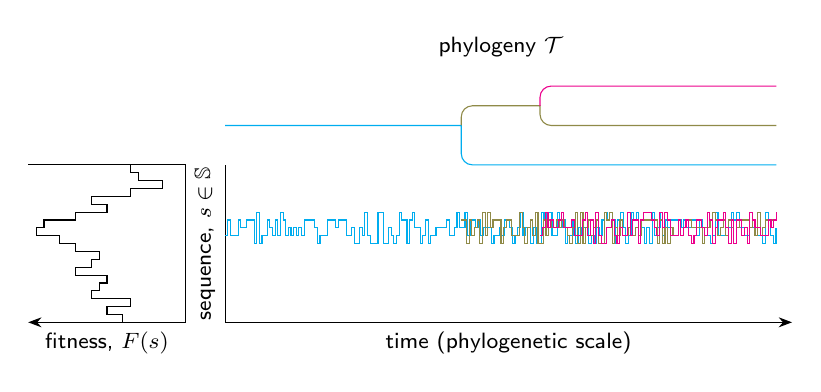
\begin{tikzpicture}[font=\footnotesize]

\draw[-Stealth] (0,-1) -- node[anchor=north] {time (phylogenetic~scale)} (7.2,-1) ;
\draw[xshift=-0.0 cm] (0,-1) -- node[rotate=90, anchor=south]
{sequence, \(s\in\mathbb{S}\)} (0,1) ;
\draw[-Stealth, xshift=-0.5 cm] (0,-1) -- node[anchor=north] {fitness, \(F(s)\)} (-2,-1) ;
\draw[xshift=-0.5 cm] (0,1) -- (-2,1) ;
\draw[xshift=-0.5 cm] (0,-1) -- (0,1) ;

% fitness landscape
\draw[rotate=90, yshift=0.5 cm] plot[const plot] coordinates {
(-1.0,0.8) (-0.9,1.0) (-0.8,0.7) (-0.7,1.2) (-0.6,1.1) (-0.5,1.0) (-0.4,1.4) (-0.3,1.2) (-0.2,1.1) (-0.1,1.4) (0.0,1.6) (0.1,1.9) (0.2,1.8) (0.3,1.4) (0.4,1.0) (0.5,1.2) (0.6,0.7) (0.7,0.3) (0.8,0.6) (0.9,0.7) (1.0,0.7)
};

% evol. trajectories

\draw[
cyan,
domain=0:7, samples=210]
plot[const plot] (\x, {round((0.2 * rand + 0.2) * 10) / 10 }) ;
\path
(3.5,0.2) coordinate (zoomleft)
(3.6,0.2) coordinate (zoomright)
;

\draw[
yellow!50!black,
domain=3:7, samples=120]
plot[const plot] (\x, {round((0.2 * rand + 0.2) * 10) / 10 }) ;
\path
(3.5,0.2) coordinate (zoomleft)
(3.6,0.2) coordinate (zoomright)
;

\draw[
magenta,
domain=4:7, samples=90]
plot[const plot] (\x, {round((0.2 * rand + 0.2) * 10) / 10 }) ;
\path
(3.5,0.2) coordinate (zoomleft)
(3.6,0.2) coordinate (zoomright)
;

\begin{scope}[yshift=1.5 cm]
\draw[cyan] (0,0) -- (3,0){[rounded corners] -- (3,-0.5) -- (7,-0.5)};
\draw[yellow!50!black] (3,0){[rounded corners] -- (3,0.25)} --
(4,0.25){[rounded corners] -- (4,0.00) -- (7,0.00)};
\draw[magenta] (4,0.25){[rounded corners] -- (4,0.5) -- (7,0.5)};
\node at (3.5,1) {phylogeny \(\mathcal{T}\)};
\end{scope}


\end{tikzpicture}

\end{document}
